
% !TEX encoding = UTF-8 Unicode

\documentclass[twocolumn,11pt,a4j]{ltjsarticle}
\usepackage{kougai}
\usepackage{siunitx}
\renewcommand{\figurename}{Fig}

\title{音響プロジェクターのための音場測定\thanks{Sound field measurement for Acoustic Projector. by MATSUMURA TAIGA (Chiba Institute of Technology)}
}
\author{〇松村 泰河 (千葉工大)}
\date{}

\begin{document}

\maketitle


\section{はじめに}
%背景
現代では音響分野のオーディオ技術が著しく成長している\cite{yamamoto2006}.
例を挙げると,5.1chや7.1ch等の多チャンネルでの視聴が可能となっているHD-DVD・Blu-ray Discの登場や,自宅で映画鑑賞などが可能となるホームシアターの普及がある.
音響技術の発展により,音波を聴取者の位置に向けることで臨場感を持たせることが可能となっている.

%問題点
5.1chや7.1ch等のサラウンド環境は,聴取者が最適な位置にいる場合のみを想定したスピーカーの配置が研究されている\cite{kurosumi1994}.
そのため,位置や体勢を変えるなど,複数人での利用は想定されていない.
また,サラウンド環境では映像内の話者の位置と実際の音の位置に差がある.
その問題を改善することを目的としてオーセンサラウンドが開発された\cite{authensurround}.
オーセンサラウンドは,ディスプレイから出る音声に音像定位を利用した信号を加えることで,映像内の話者の位置と実際の音の位置の差を無くして臨場感を持たせることができる音響機器である.
しかし,オーセンサラウンドは大画面には対応していないという問題点がある.
また,SONY社に360 Reality Audioという技術がある\cite{360RealityAudio}.
この技術は,SONY社の360立体音響技術を使用しており,ヘッドホンで立体的な音場を体感することができる.
しかし,360 Reality Audioはヘッドホンでの使用を目的としているため複数人での聴取をすることができない.


%提案
これらの問題点を解決するために,聴取者が最適な位置にいなくてもスクリーン上の話者の口元等に仮想音源を置き,臨場感を持たせる機器の開発を考案する.
%目的
この機器を音響プロジェクターと呼び,音響プロジェクターの実現に向けて,音場を測定することを目的とする.

\section{音響プロジェクターの構想}
Fig.\ref{fig:音響プロジェクター}は音響プロジェクターを用いた際の使用イメージである.
鋭い指向性の音波を画面上の対象の話者の口元に当て,その仮想音源の位置から音が広がるような仕組みである.
理想状態では,スクリーン上の仮想音源から音が広がっているような感覚となっているため,聴取者は位置を縛られず,複数人での聴取が可能となる.

本研究の最終的な目的としては,鋭い指向性の音波を画面に反射させることで,聴取者の位置によらず大画面でも臨場感のある音場環境を作ることである.

\vspace{1ex}
\begin{figure}[h]
\begin{center}
 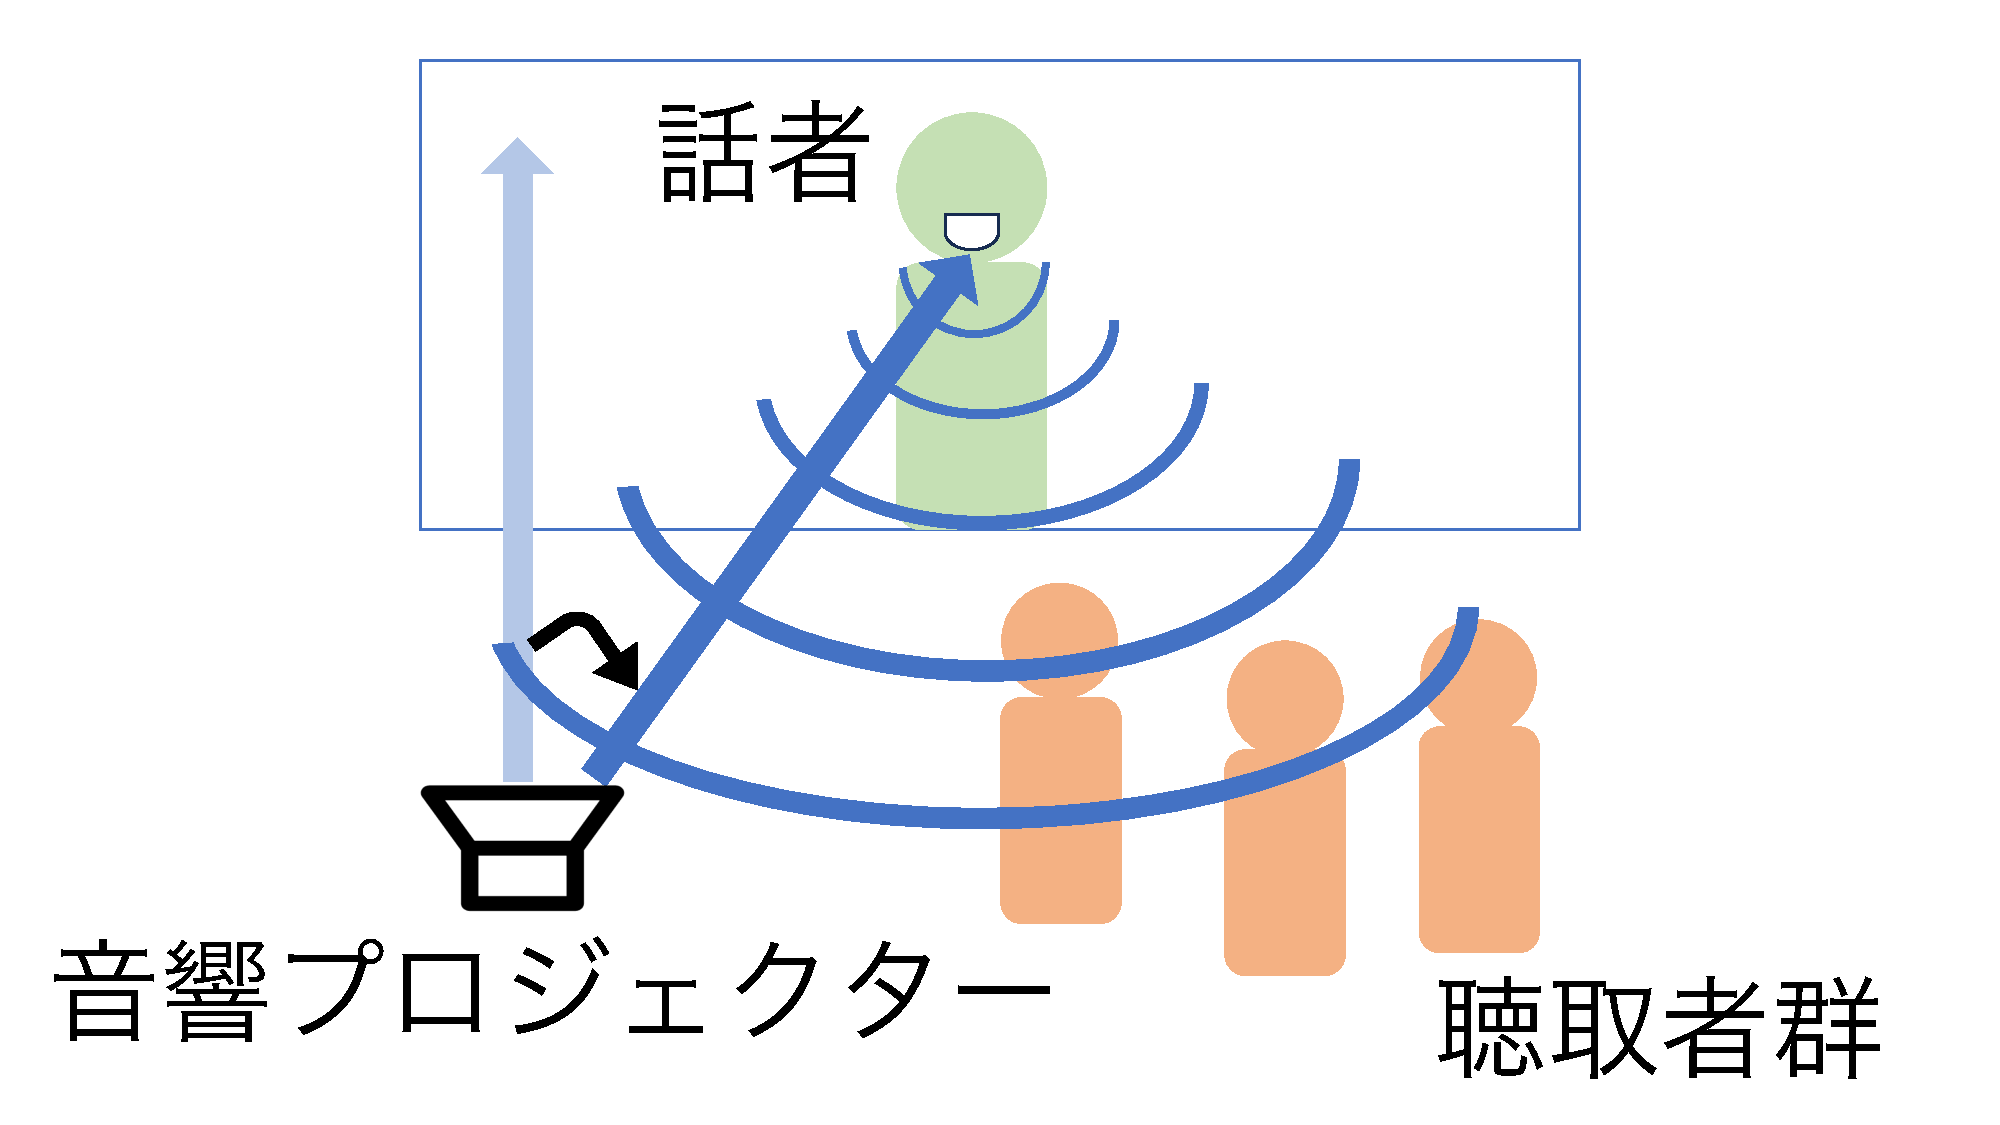
\includegraphics[clip,width=80mm,height=50mm]{onkyouP.pdf}
\end{center}
 \caption{音響プロジェクターの使用イメージ}
 \label{fig:音響プロジェクター}
\end{figure}



\section{音響プロジェクターの実現のための音場測定}

一般的に鋭い指向性を作る方法として,音響ホーンやスピーカーアレイが知られている.
そこで,本研究ではこれらの機器を使用し,鋭い指向性を持つ音波をスクリーンにあてて,音場を測定する.

音響プロジェクターの実際の使用を想定して音場の測定を行なった.
音場測定は,まず,指向性スピーカーを用いて鋭い指向性を持つ音波を生成し,スクリーンに向けて音波を反射させる.
次に,反射後の音波をオシロスコープにつなげたマイクで音圧の測定を行う.
本研究の実験では,スクリーンと指向性スピーカーの距離と等しい距離にマイクを置いて,マイクを$\ang{10}$から$\ang{170}$の位置に$\ang{5}$ずつ移動させることで,各角度の音圧を測定し,音場を可視化している.
また,指向性スピーカーは$\ang{0}$・$\ang{15}$・$\ang{30}$に移動させて,音源の角度による音場を計測することで各角度での比較を行えるようにしている.

%変更を加える

Fig.\ref{fig:結果}にスピーカーアレイで2000 Hzと8000 Hzの周波数を出し,音源は$\ang{90}$配置して音波を出す.
この図から,音源が$\ang{90}$のとき入射角と反射角が$\ang{0}$であり,$\ang{90}$付近の音圧が高くなっている.
2000 Hzは8000 Hzと比べて高い音圧であることがわかる.

\vspace{1ex}
\begin{figure}[h]
\begin{center}
 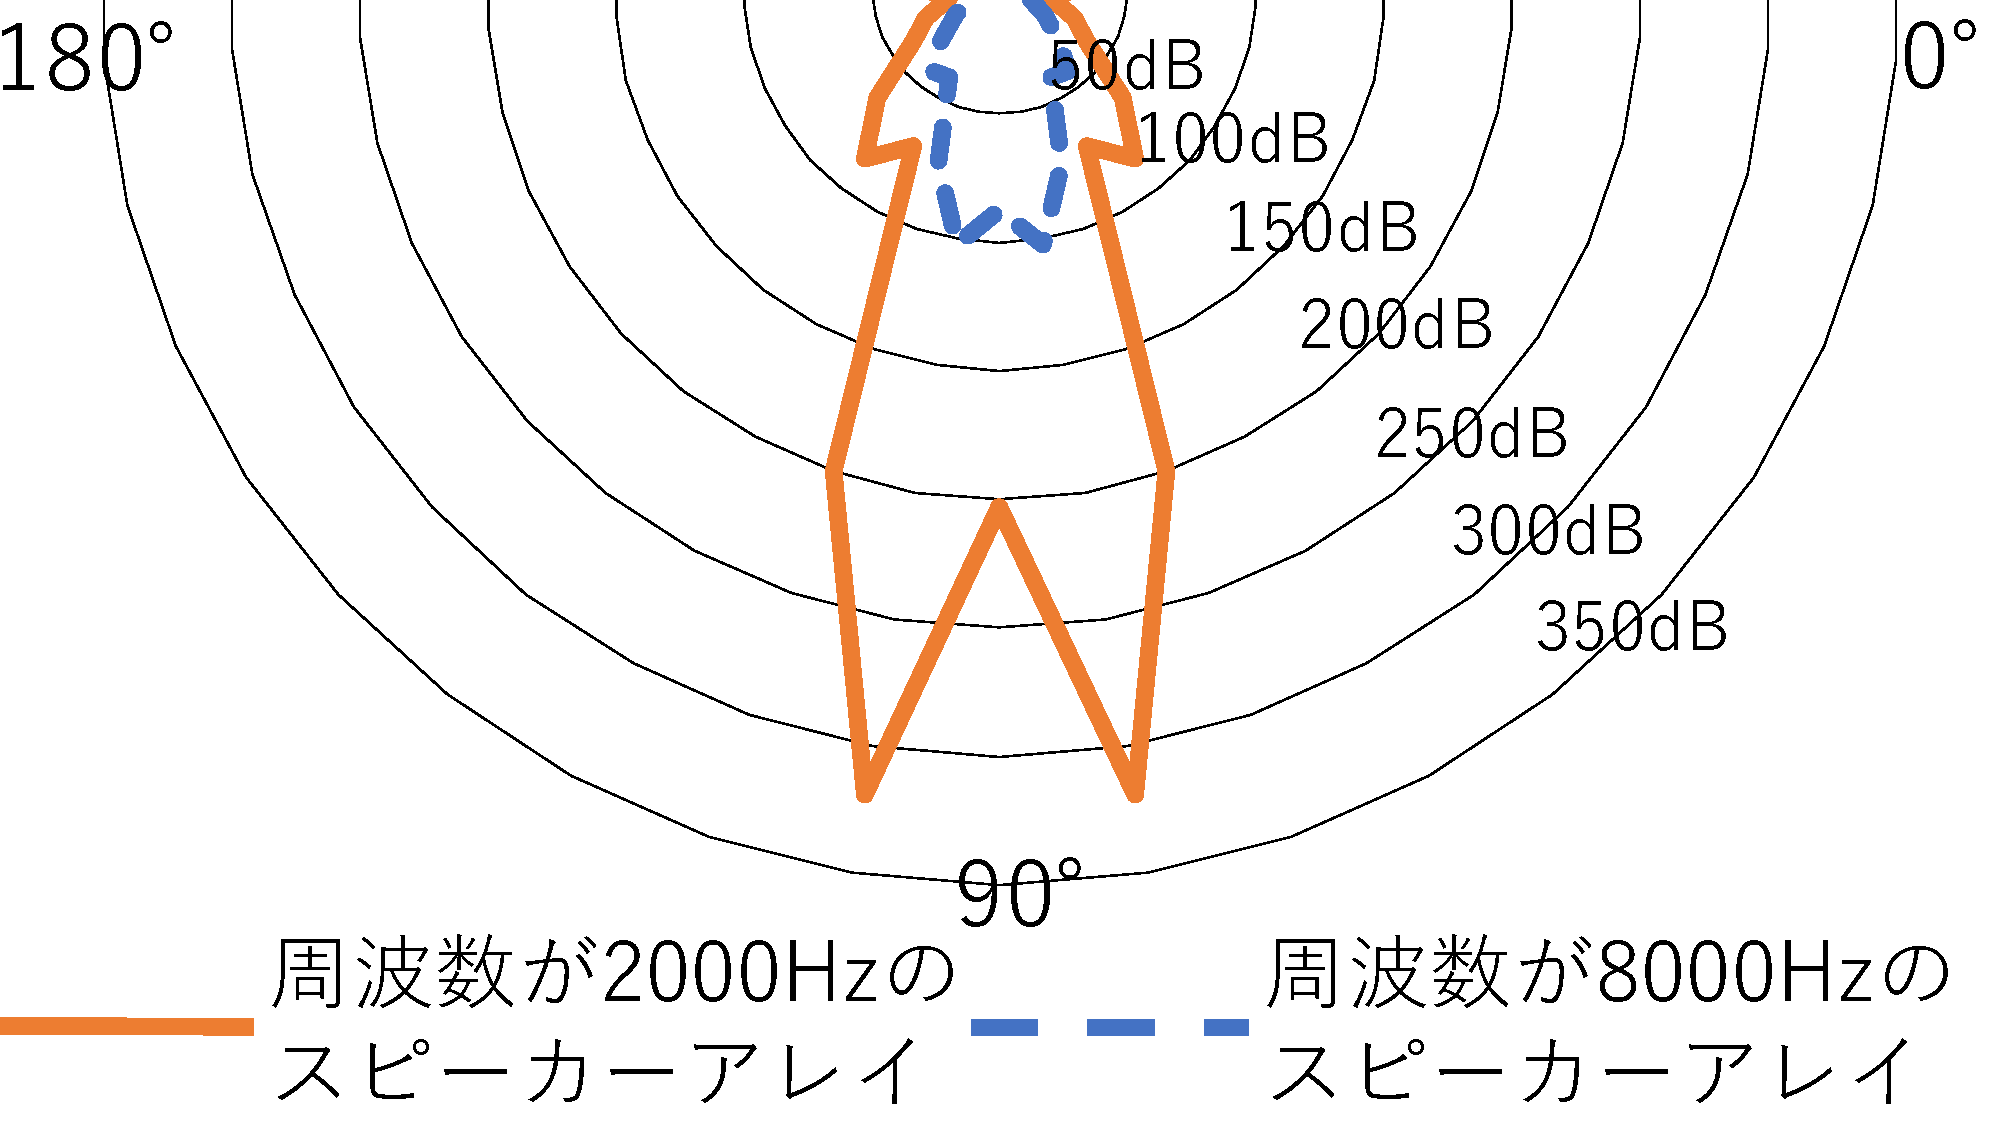
\includegraphics[clip,width=75mm,height=45mm]{keltuka4.pdf}
\end{center}
 \caption{実験結果}
 \label{fig:結果}
\end{figure}

\vspace{1ex}
Fig.\ref{fig:結果1}にスピーカーアレイで8000 Hzの周波数を出し,音源は$\ang{90}$の位置と$\ang{75}$の位置に配置して音波を出した際の比較を示す.
この図から,音源が$\ang{90}$のときは入射角と反射角が$\ang{0}$であり,$\ang{90}$付近の音圧が高くなっている.
また,音源が$\ang{75}$のときは入射角と反射角が$\ang{15}$であり,$\ang{105}$付近の音圧が高くなっている.
双方の実験結果を比較すると,同じ音源を使用しているが音圧に差があることがわかる.
これは,音源が$\ang{75}$の位置にあるときは入射波と反射波が干渉しないが,音源が$\ang{90}$の位置にある時は音波が干渉してしまい音圧に差が出てしまうのではないかと考える.

\vspace{1ex}
\begin{figure}[h]
\begin{center}
 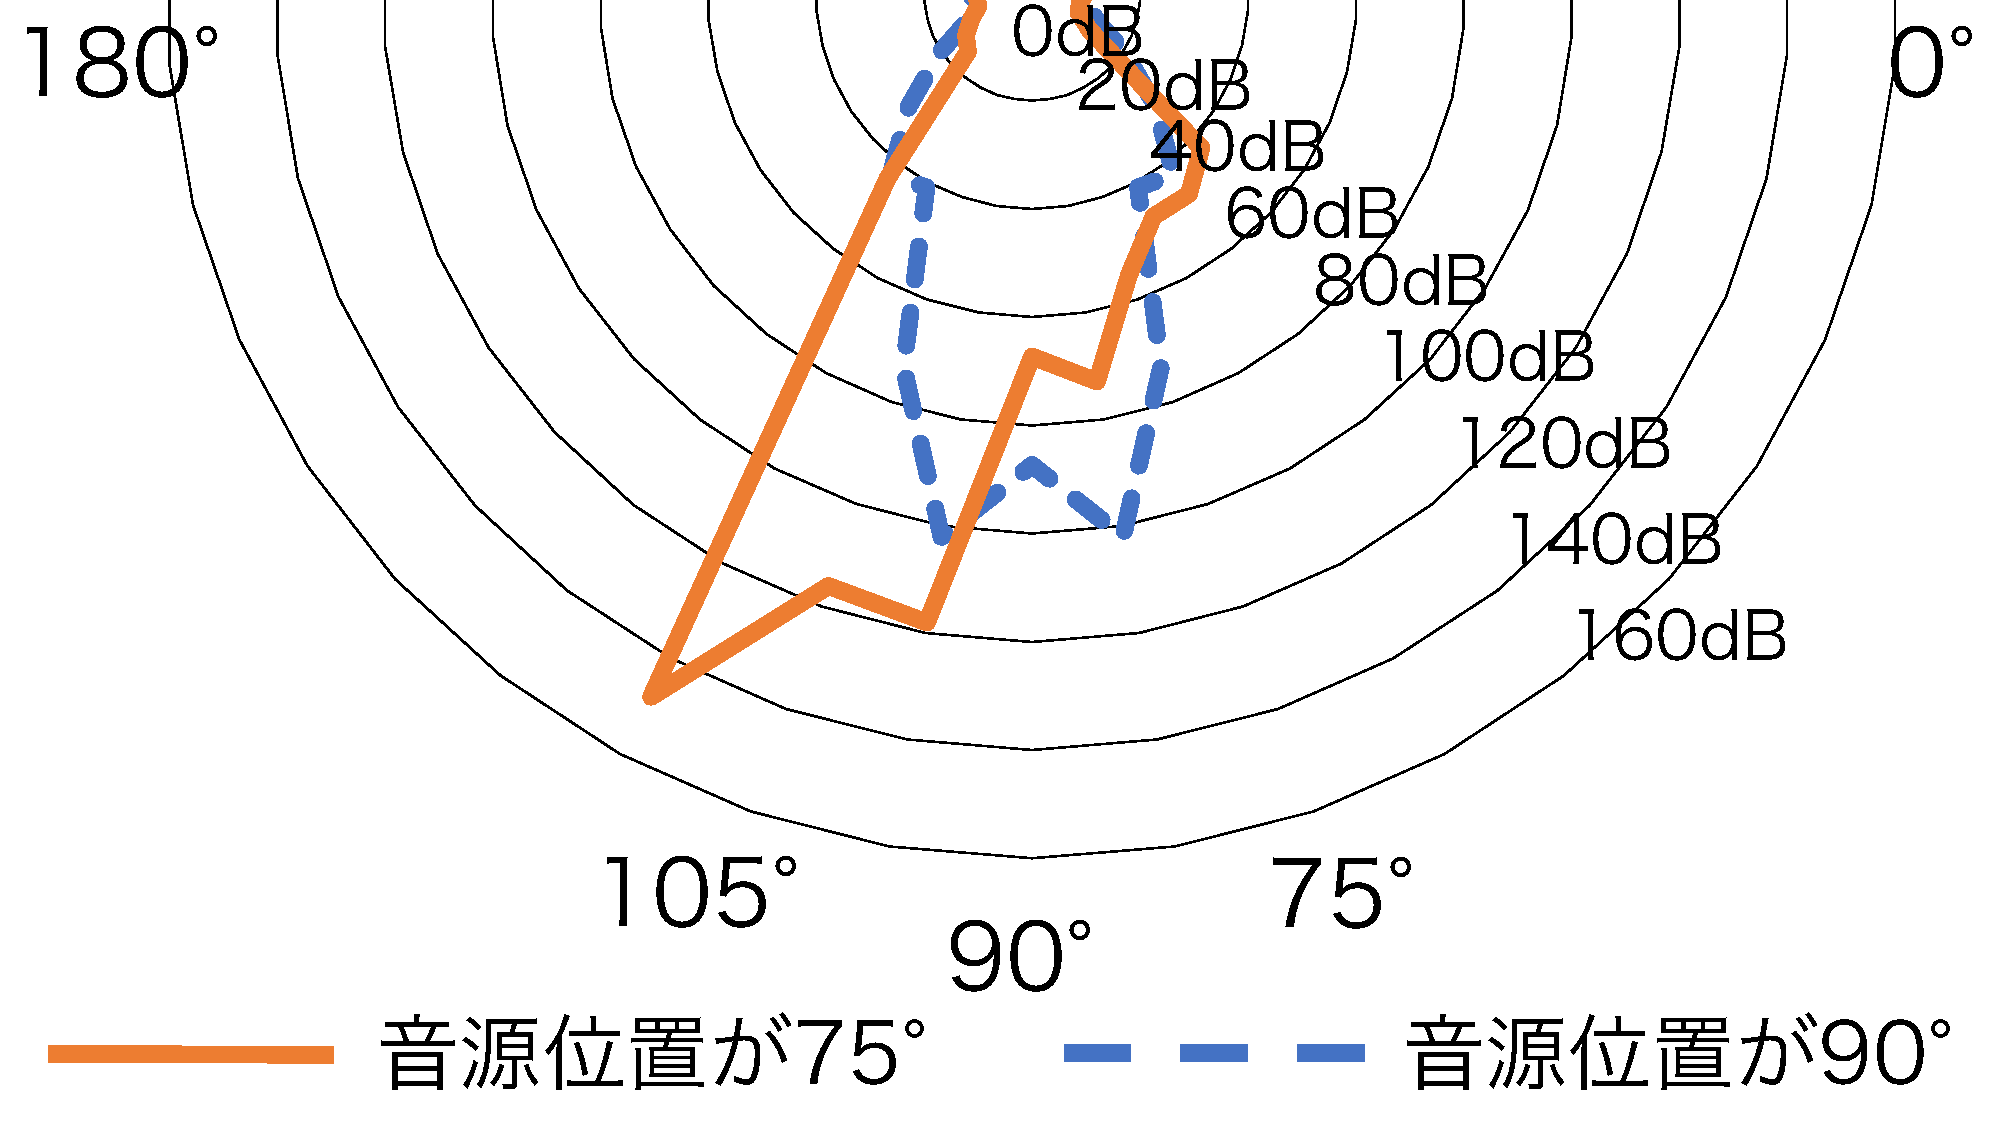
\includegraphics[clip,width=75mm,height=45mm]{keltuka.pdf}
\end{center}
 \caption{実験結果}
 \label{fig:結果1}
\end{figure}

\vspace{1ex}
Fig.\ref{fig:結果2}に音響ホーンで8000 Hzの周波数を出し,音源は$\ang{75}$の位置と$\ang{60}$の位置に配置して音波を出している.
この図から,音源が$\ang{75}$のときは入射角と反射角が$\ang{15}$であり,$\ang{105}$付近の音圧が高くなっている.
また,音源が$\ang{60}$のときは入射角と反射角が$\ang{30}$であり,$\ang{120}$付近の音圧が高くなっている.


\vspace{1ex}
\begin{figure}[h]
\begin{center}
 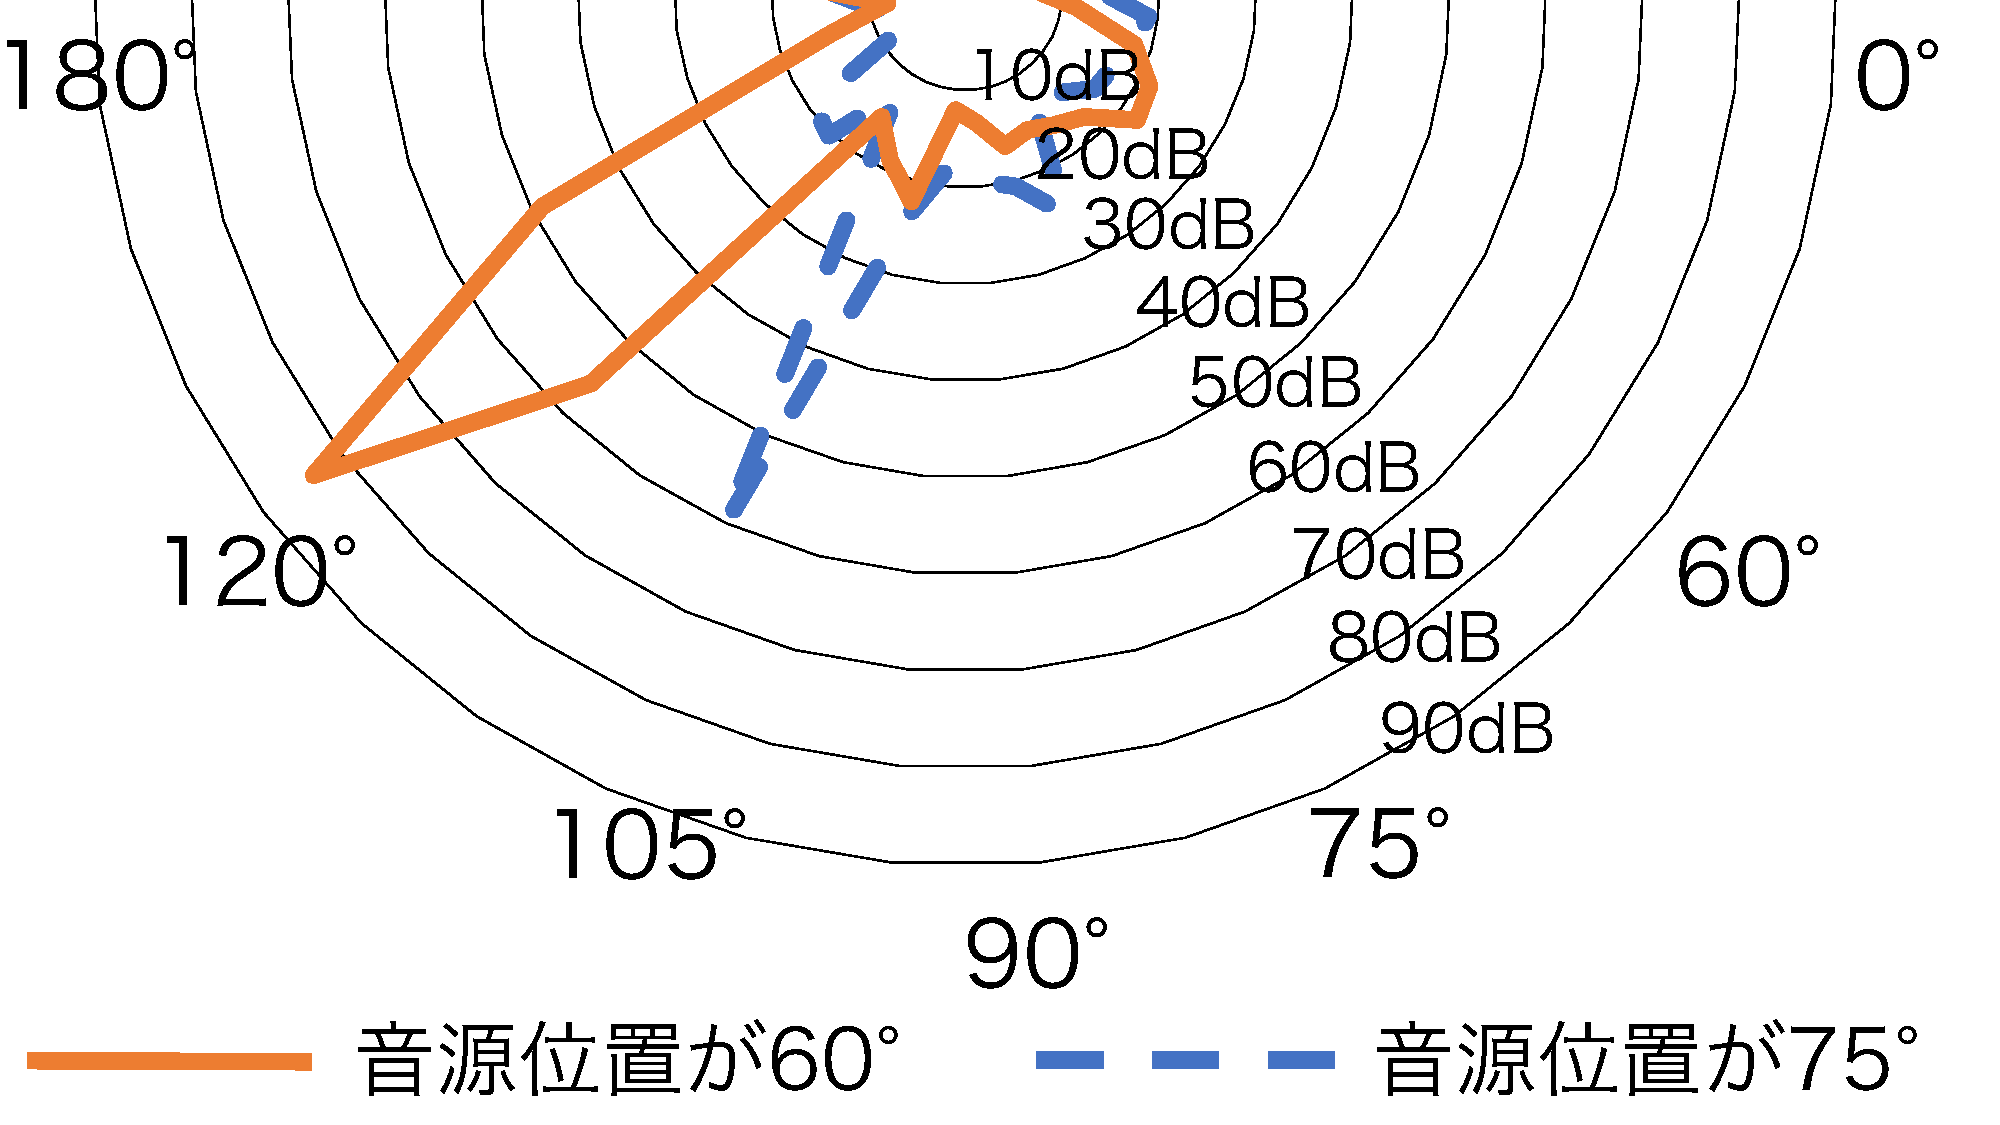
\includegraphics[clip,width=75mm,height=45mm]{keltuka2.pdf}
\end{center}
 \caption{実験結果}
 \label{fig:結果2}
\end{figure}

\vspace{1ex}
Fig.\ref{fig:結果3}は音源を$\ang{75}$の位置に配置し,スピーカーアレイと音響ホーンで音波を出している.
この図から,どちらの音源を使用しても,$\ang{105}$付近の音圧が高くなっていることがわかる.
また,本研究の実験結果では音響ホーンとスピーカーアレイを比較すると,スピーカーアレイから高い音圧を得られることがわかった.
一方,本研究で使用した音響ホーンはスピーカーアレイと同等の大きさであり,比較すると指向性が鋭いが音圧が低い.


\vspace{1ex}
\begin{figure}[h]
\begin{center}
 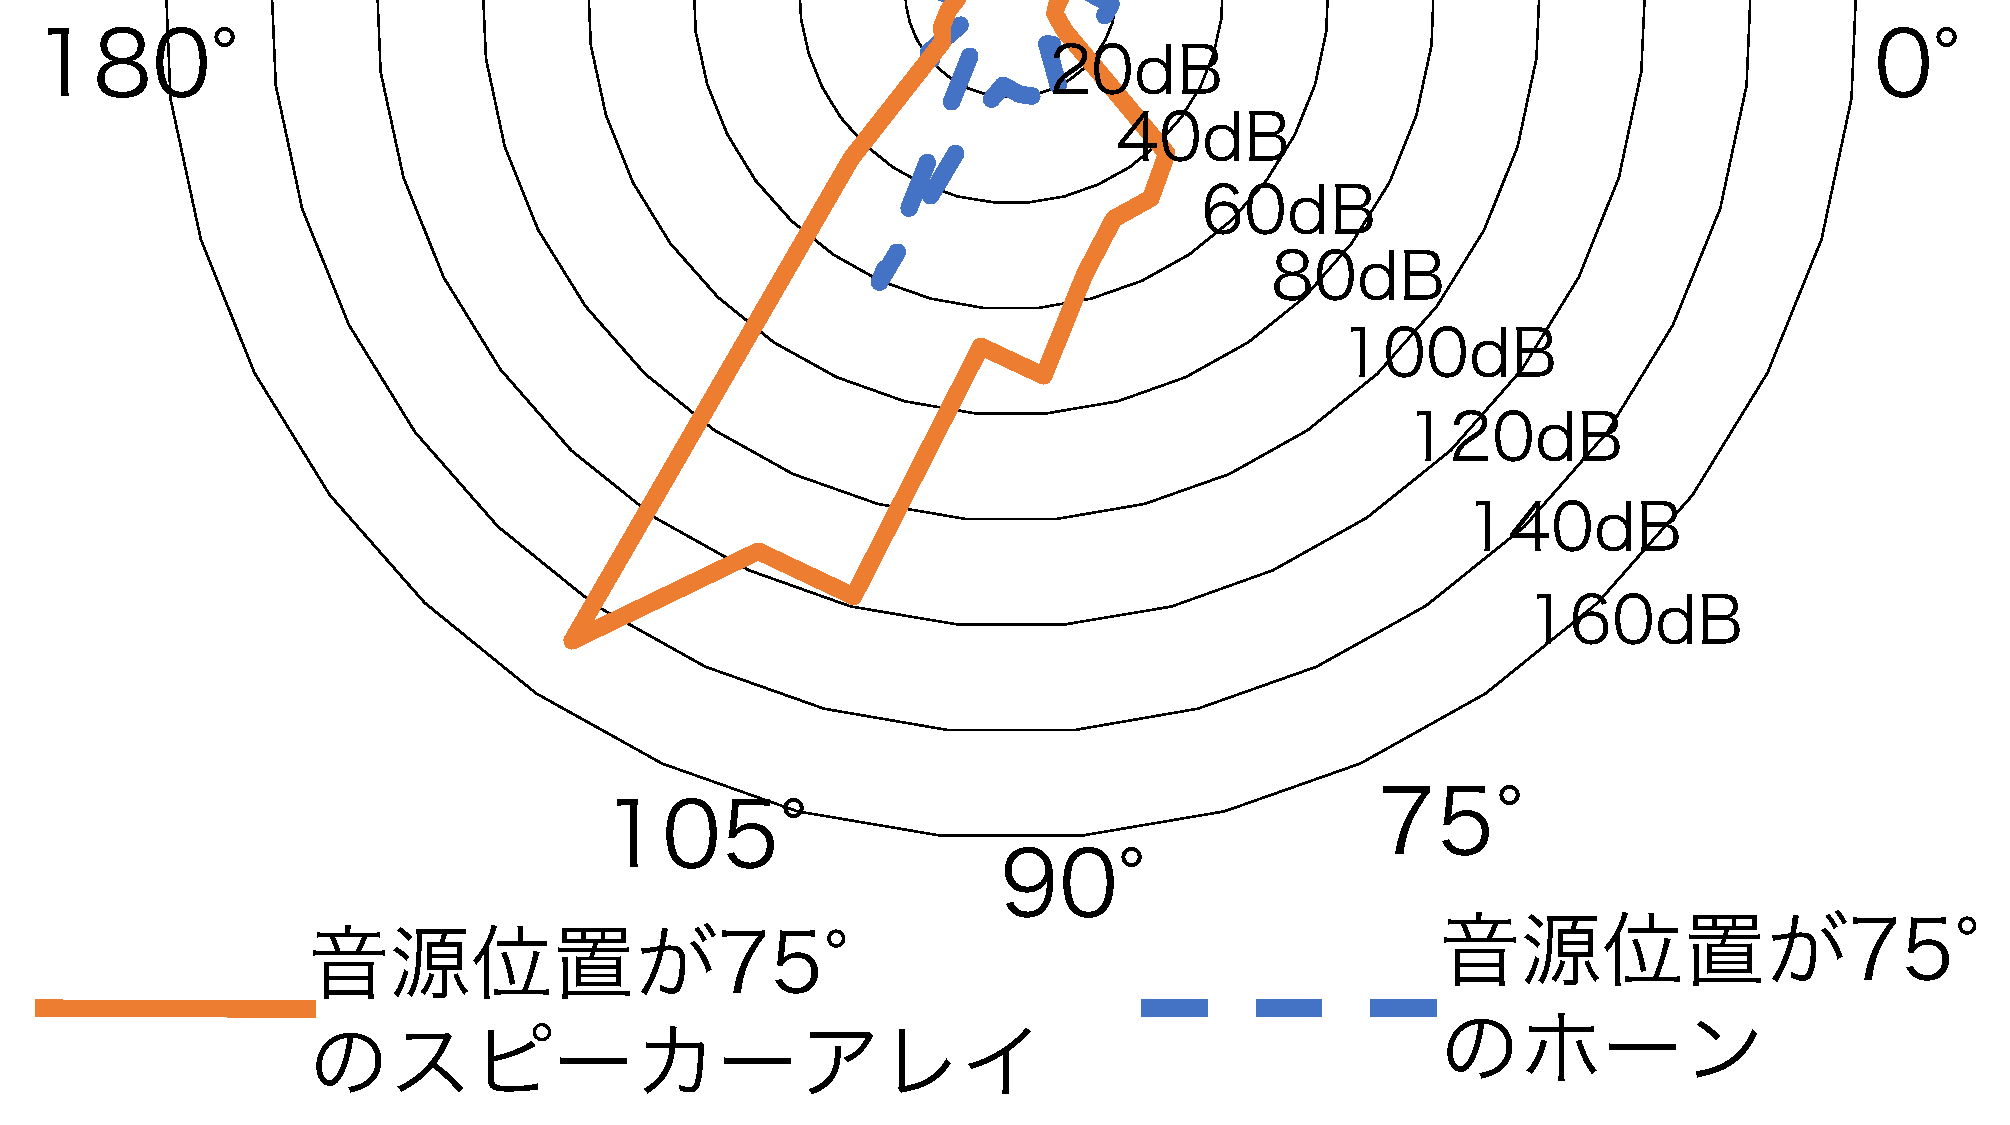
\includegraphics[clip,width=75mm,height=45mm]{keltuka3.pdf}
\end{center}
 \caption{実験結果}
 \label{fig:結果3}
\end{figure}

\vspace{1ex}
Fig.\ref{fig:結果},\ref{fig:結果1},\ref{fig:結果2},\ref{fig:結果3}から周波数や音源を変更しても音波の大部分では幾何光学的に反射していることがわかる.
理想状態では音波が仮想音源から音波が均等に広がってほしいのだが,音波が幾何光学的に反射してしまっているため,現在の指向性スピーカーをそのまま使用することは難しい.

\vspace{1ex}
\section{おわりに}
本研究では,鋭い指向性を持つ音波をスクリーンに反射させて音場を測定した.
そこで音波は幾何光学的に反射する成分が大きいことがわかった.
この測定結果を活用して音響プロジェクターの実現を目指していく.

\vspace{1ex}
\paragraph{謝辞}
本研究にあたりご指導くださった須田宇宙先生,実験環境を提供していただいた高橋義典先生に感謝申し上げます.

\begin{thebibliography}{99}
\bibitem{yamamoto2006} 山本貢平: "音響学の行方'',日本音響学会誌,62巻1号 (2006) ,pp.1−2, 2023/12/29参照
\bibitem{kurosumi1994} 黒住幸一: "放送におけるメルチチャネルステレオ音声方式'',日本音響学会誌,50巻11号 (1994) ,pp.915−920, 2023/7/7参照
\bibitem{authensurround} NEC Lavie: "https://support.nec-lavie.jp/product/pc/200509/common/function/sound/authensurround/index.html", 2023/7/18参照
\bibitem{360RealityAudio} 360 Reality Audio: "https://www.sony.jp/headphone/special/360\_Reality\_Audio/", 2023/12/24参照

\end{thebibliography}


\end{document}
